\documentclass[10pt]{article}
\usepackage[margin=3cm]{geometry}
\usepackage[utf8]{inputenc}
\usepackage[english,slovak]{babel}
\usepackage{array, xcolor}
\definecolor{lightgray}{gray}{0.8}
\newcolumntype{L}{>{\raggedleft}p{0.14\textwidth}}
\newcolumntype{R}{p{0.8\textwidth}}
\newcommand\VRule{\color{lightgray}\vrule width 0.5pt}
\usepackage{bibentry}
\usepackage{hyperref}
\usepackage{graphicx}
\usepackage{multicol}

\title{\bfseries\Huge Michal Chovanec}
\author{michal.nand@gmail.com}
\date{}
\begin{document}
\maketitle





\begin{minipage}{0.5\textwidth}

	Ing. Michal Chovanec, PhD. \\
	Staničná 11\\
	Lietavská Lúčka 01311\\
	Slovakia

\end{minipage} \hfill
\begin{minipage}{0.45\textwidth}

	\begin{flushright}
	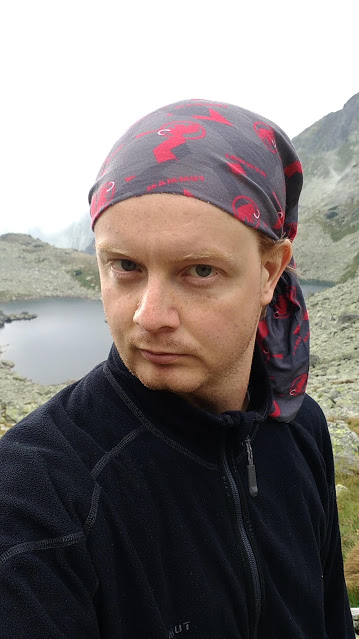
\includegraphics[width=0.5\textwidth]{photo2.jpg}
	\end{flushright}

\end{minipage}





\section*{Work experiences}
\begin{tabular}{L!{\VRule}R}
2019--today& Tachyum - AI research (C++, Pytorch, BLAS libs) \\
2018--2019& Research on Faculty of management science and informatics \\
	&Cell in fluid - red blood cells trajectory prediction using deep neural networks  \\ [5pt]
	&Deep reinforcement learning (deep Q networks, curiosity learning) ATARI, DOOM, Go games \\ [5pt]
2016--2018& Research on Faculty of management science and informatics \\
 	& Artifical inteligence and learning systems  \\ [5pt]
	& Deep reinforcement learning for GO game using dense CNN \\ [5pt]
	& Dense net implementations on embedded system \\ [5pt]
2015--2016& Ceit group, Žilina \\
		  & ZIMS department, AGV robotics navigation research and development  \\ [5pt] \\
2012--2013& Scheidt\&Bachmann, Žilina \\
		  & Bahn department, railway security (solutions) systems (Visual C++ programming)

\end{tabular}


\section*{Education}
\begin{tabular}{L!{\VRule}R}
2013--2016& PhD degree : Faculty of management science and informatics, University of Žilina \\
  & PhD thesis : Function approximation in Q-learning algorithms \\
2011--2013& Master degree : Faculty of management science and informatics, Computer engineering, Ing. (Msc.) \\
	& Diploma thesis : Operational system for arm cortex-m3 (stm32)\\
2007--2011& Bachelor degree : Faculty of management science and informatics, Computer engineering Bc. \\
	& Bachelor thesis : FPGA audio player (Xilinx FPGA)
\end{tabular}

\section*{Deep learning skills}
\begin{tabular}{L!{\VRule}R}
reinforcement learning & DQN, dueling DQN, attention in DQN, rainbow, actor critic, a2c \\
image processing & segmentation, classification (FastSCNN, FCN, U-Net, Resnet) \\
basics in signal processing & digital filter design, FFT, LSTM, GRU, Temporal CNN \\
own DL framework & C++, Cuda, Python\\
\end{tabular}

\section*{Computer skills}
\begin{tabular}{L!{\VRule}R}
expert & C, C++, Python\\
basic & Ruby, VHLD, Java \\
tools & GNU GCC, G++, NVCC, Make, Gnuplot, Sublime, Atom, dfu-util \\
technologies & NVIDIA Cuda, OpenMPI, OpenGL, OpenCV, Numpy, Scipy, JsonCpp, CImg \\
embedded & ARM Cortex M0..M7 (stm32), msp430, avr \\
other & real time systems, artificial intelligenc (deep learning, reinforcement learning), robotics, inertial nevigation, controll theory, adaptive and learning systems
\end{tabular}


\section*{Rewards}
\begin{tabular}{L!{\VRule}R}

2019 & CodersRank, worldwide : C++ top 2\%, Cuda top 7\%, Python top 2\%,
	\href{https://profile.codersrank.io/user/michalnand}{link} \\
2016 & Istrobot Line Follower L2 cathegory first place (robotics competition) \\
2013 & Master degree with honors \\
 & Dean price for best diploma thesis \\
 & ACM Certificate Gallery of the best \\
 & Soit price for open sources diploma thesis, 3rd place \\
2011 & Dean price for best bachelor thesis
\end{tabular}


\bibliographystyle{plain}
\nobibliography{publication.bib}
\section*{Publications}
\begin{tabular}{L!{\VRule}R}

2012 & $[1]$ Preemptívny multitasking pre mikrokontroléry s jadrom ARM Cortex M3 Michal Chovanec. - 2012 In: Otvorený softvér vo vzdelávaní, výskume a v IT riešeniach S. 27-32 zborník príspevkov medzinárodnej konferencie OSSConf 2012 2.-4. júla 2013 Žilina, Slovensko Bratislava Spoločnosť pre otvorené informačné technológie 2012, ISBN 978-80-970457-2-2 \\[5pt]
2013 & $[2]$ Akcelerometrické meranie výstrelu z luku Michal Chovanec a Jaroslav Múčka. - 2013 In: Otvorený softvér vo vzdelávaní, výskume a v IT riešeniach S. 39-46 zborník príspevkov medzinárodnej konferencie OSSConf 2013 2.-4. júla 2013 Žilina, Slovensko Bratislava Spoločnosť pre otvorené informačné technológie 2013, ISBN 978-80-970457-3-9 \\[5pt]
& $[3]$ Wireless sensor networks for intelligent transportation systems Michal Hodoň, Juraj Miček, Michal Chovanec. - 2013 In: IEEE CommSoft E-Letters Vol. 2, no. 1, (2013), online, s. 3-8 elektronický zdroj \\[5pt]
& $[4]$ Intelligent traffic-safety mirror, M. Hodon, M. Chovanec, M. Hyben, 2013 In: Studia Informatica Universalis - 2013, volume 11/1 \\[5pt]
2014 & $[5]$ Universal synchronization algorithm for wireless sensor networks - "FUSA algorithm" / Michal Chovanec ... [et al.].
In: FedCSIS : proceedings of the 2014 federated conference on Computer science and information systems : September 7-10, 2014, Warsaw, Poland. - Los Alamitos; Warsaw: IEEE; Polskie Towarzystwo Informatyczne, 2014. - ISBN 978-83-60810-61-3. - S. 1001-1007.
 \\[5pt]
& $[6]$ Tiny low-power WSN node for the vehicle detection [Jednoduchý energeticky-efektívny nód bezdôtovej senzorovej siete určený na detekciu automobilov] / Michal Chovanec, Michal Hodon and Lukas Cechovic. \\[5pt]
& $[7]$ Investigation of the gyro-sensor contribution to the straight movement of vehicle [Analýza vplyvu gyroskopického senzora pri priamom pohybe vozidla] / Michal Hodoň, Michal Chovanec.  \\[5pt]
2015 & $[8]$ Required value classification using Kohonen neural network = Klasifikácia žiadanej hodnoty Kohonenovou neurónovou sieťou / Michal Chovanec.
In: Otvorený softvér vo vzdelávaní, výskume a v IT riešeniach : zborník príspevkov medzinárodnej konferencie OSSConf 2015 : 1.-3. júla 2015 Žilina, Slovensko. - Žilina: Žilinská univerzita, 2015. - ISBN 978-80-970457-7-7. \\[5pt]
2016 & $[9]$ Water level monitoring based on the acoustic signal using the neural network / Veronika Olesnanikova, Karpiš Ondrej, Chovanec Michal, Šarafín Peter, Žalman Róbert
In: Information and digital technologies 2016 proceedings of the international conference : 5-7 July 2016 Rzeszow, Poland. - [S.l.]: IEEE, 2016. - ISBN 978-1-4673-8860-3  \\[5pt]
& $[10]$ Aeris Robots Laboratory with Dynamic Environment / Michal Chovanec, Lukáš Čechovič, Lukáš Mandák, Robotics in Education Research and Practices for Robotics in STEM Education ISBN: 978-3-319-42974-8 (Print) 978-3-319-42975-5 (Online), pages 169-180  \\[5pt]
2018 & $[11]$ Simulation of blood flow in microfluidic devices for analysing of video from real experiments / Hynek Bachratý, Katarína Bachratá, Michal Chovanec, František Kajánek, Monika Smiešková, Martin Slavík \\[5pt]
2019 & $[12]$ Convolutional neural networks for red blood cell trajectory prediction in simulation of blood flow / Michal Chovanec, Hynek Bachratý, Katarína Bachratá, Katarína Jasenčáková, Cham: Springer Nature, ISBN 978-3-030-17934-2
\end{tabular}

\newpage
\section*{Active projects}

Active projects in deep learning field, including sources on github and some videos

\begin{itemize}

\item \href{https://github.com/michalnand/reinforcement_learning}{Reinforcement learning experiments \\
	https://github.com/michalnand/reinforcement\_learning}

\item \href{https://www.youtube.com/watch?v=rQIShnTz1kU}{Reinforcement learning video \\
	https://www.youtube.com/watch?v=rQIShnTz1kU}

\item \href{https://github.com/michalnand/reinforcement_learning_tutorial}{Reinforcement learning workshop \\
	https://github.com/michalnand/reinforcement\_learning\_tutorial}

\item \href{https://github.com/michalnand/rysy/tree/master/rysy2}{Own convolutional neural networks framework \\
	https://github.com/michalnand/rysy/tree/master/rysy2}


\end{itemize}

\section*{Robotics projects}
Line following robot for competition using neural networks for line shape prediction.
\begin{itemize}
\item \href{https://github.com/michalnand/motoko\_uprising}{source code https://github.com/michalnand/motoko\_uprising}
\item \href{https://hackaday.io/project/163799-motoko-uprising-deep-neural-network-line-following}{Line following robot - Post on hackaday blog}
\item \href{https://hackaday.io/project/19924-self-learning-robot}{Self learning robot - Post on hackaday blog}
\item \href{https://www.youtube.com/watch?v=E9FJIDowNmU}{video : https://www.youtube.com/watch?v=E9FJIDowNmU}
\item \href{https://www.youtube.com/watch?v=8sskJN\_zuko}{video : https://www.youtube.com/watch?v=8sskJN\_zuko}
\item \href{https://www.youtube.com/watch?v=xXKnUeN1VgI}{video : https://www.youtube.com/watch?v=xXKnUeN1VgI}
\item \href{https://www.youtube.com/watch?v=UDmeS721\_-Q}{video from competition : https://www.youtube.com/watch?v=UDmeS721\_-Q}
\end{itemize}

\section*{Diploma and PhD final projects}
Diploma thesis : Real time operating system for Cortex M3
\begin{itemize}
\item \href{https://github.com/michalnand/suzuha\_os}{source code : https://github.com/michalnand/suzuha\_os}
\item \href{https://fedcsis.org/proceedings/2015/pliks/146.pdf}{publication : https://fedcsis.org/proceedings/2015/pliks/146.pdf}
\end{itemize}
Dissertation thesis : Q function approximation in Q-learning algorithms
\begin{itemize}
\item \href{https://github.com/michalnand/q\_learning}{source code : https://github.com/michalnand/q\_learning}
\item \href{https://github.com/michalnand/q\_learning/blob/master/doc/presentation\_march\_2016\_ktk/presentation.pdf}{summary : https://github.com/michalnand/q\_learning/blob/master/doc\\
                  /presentation\_march\_2016\_ktk/presentation.pdf}
\end{itemize}

\section*{Interests}
robotics (artificial intelligence, real time controll),
outdoor (hiking, running, bouldering, caving, survival and critical situations),
martial arts (archery, aikido, kenjutsu), music, yoga

\end{document}
